\uuid{yPMg}
\exo7id{5091}
\titre{exo7 5091}
\auteur{rouget}
\organisation{exo7}
\datecreate{2010-06-30}
\isIndication{false}
\isCorrection{true}
\chapitre{Fonctions circulaires et hyperboliques inverses}
\sousChapitre{Fonctions hyperboliques et hyperboliques inverses}
\module{Analyse}
\niveau{L1}
\difficulte{}

\contenu{
\question{
Etudier $f~:~x\mapsto\ln(\ch x)-x$.
}
\reponse{
\textbullet~Pour tout réel $x$, $\ch x>0$. Donc $f$ est définie, continue et dérivable sur $\Rr$. Pour tout réel $x$,

\begin{center}
$f'(x)=\sh x\frac{1}{\ch x}-1=\tanh x-1<0.$
\end{center}
$f$ est donc strictement décroissante sur $\Rr$.
\textbullet~Etude en $-\infty$. $\lim_{x\rightarrow -\infty}\ch x=+\infty$ et donc $\lim_{x\rightarrow -\infty}f(x)=+\infty$.
Cherchons une éventuelle droite asymptote.

\begin{center}
$f(x)=\ln\frac{e^x+e^{-x}}{2}-x=\ln(e^x+e^{-x})-\ln2-x=\ln(e^{-x})-x-\ln2+\ln(1+e^{2x})=-2x-\ln2+\ln(1+e^{2x}).$
\end{center}
Donc, $f(x)-(-2x-\ln2)=\ln(1+e^{2x})$. Or, d'une part $\lim_{x\rightarrow -\infty}\ln(1+e^{2x})= 0$ et donc la droite
$(D)$ d'équation $y=-2x-\ln2$ est asymptote à la courbe représentative de $f$ en $-\infty$ et d'autre part, pour
tout réel $x$, $\ln(1+e^{2x})>0$ et la courbe représentative de f est strictement au dessus de $(D)$ sur $\Rr$.
\textbullet~Etude en $+\infty$.
\begin{center}
$f(x)=\ln\frac{e^x+e^{-x}}{2}-x=\ln(e^x+e^{-x})-\ln2-x=\ln(e^x)-x-\ln2+\ln(1+e^{-2x})=-\ln2+\ln(1+e^{-2x})$
\end{center}
et $f$ tend vers $-\ln2$ quand $x$ tend vers $+\infty$.
\textbullet~Graphe.

$$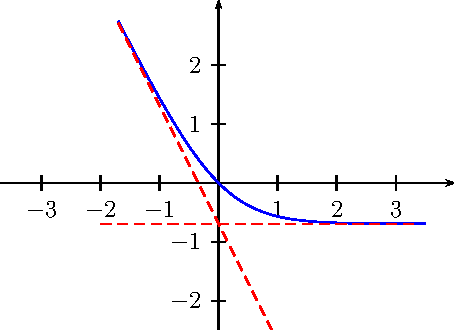
\includegraphics{../images/pdf/yPMg-1.pdf}$$
}
}
